\documentclass[tikz,border=8pt,multi=tikzpicture]{standalone}
\usepackage{amsmath}
\usepackage{xcolor}
\usetikzlibrary{arrows.meta, angles, quotes, calc}

\definecolor{mainblue}{HTML}{001158}
\definecolor{accent}{HTML}{8592bc}
\definecolor{lightaccent}{HTML}{e7e9f2}

\tikzset{
  force/.style={-{Stealth[length=3mm]}, line width=1.2pt, color=mainblue},
  dim/.style={-{Stealth[length=2mm]}, line width=0.7pt, color=accent},
  every node/.append style={font=\sffamily}
}

\begin{document}

% ---------- Figure 1: ring with two cables and hanging weight ----------
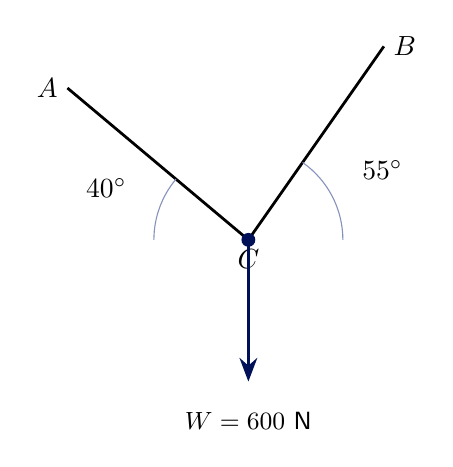
\begin{tikzpicture}
\coordinate (C) at (0,0);
\coordinate (A) at (140:3);
\coordinate (B) at (55:3);
\coordinate (Right) at ($(C)+(1,0)$);
\coordinate (Left) at ($(C)+(-1,0)$);
\draw[line width=1pt] (A) -- (C);
\draw[line width=1pt] (B) -- (C);
\fill[mainblue] (C) circle (2.5pt);
\node[left] at (A) {$A$};
\node[right] at (B) {$B$};
\node[below] at (C) {$C$};
\pic[draw=accent, angle radius=12mm, "$40^\circ$", angle eccentricity=1.6] {angle=A--C--Left};
\pic[draw=accent, angle radius=12mm, "$55^\circ$", angle eccentricity=1.6] {angle=Right--C--B};
\draw[force] (C) -- ++(0,-1.8);
\node at (0,-2.3) {\small $W = 600\ \text{N}$};
\end{tikzpicture}

% ---------- Figure 2: three concurrent forces at a point ----------
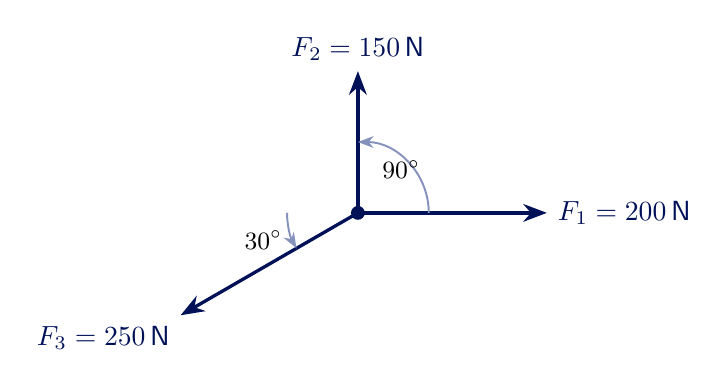
\begin{tikzpicture}
\coordinate (O) at (0,0);
\fill[mainblue] (O) circle (2.5pt);
\draw[force] (O) -- (2.4,0) node[right] {$F_1 = 200\,\text{N}$};
\draw[force] (O) -- (0,1.8) node[above] {$F_2 = 150\,\text{N}$};
\draw[force] (O) -- (210:2.6) node[below left] {$F_3 = 250\,\text{N}$};
\draw[dim] (0.9,0) arc (0:90:0.9);
\node at (0.55,0.55) {\small $90^\circ$};
\draw[dim] (180:0.9) arc (180:210:0.9);
\node at (196:1.25) {\small $30^\circ$};
\end{tikzpicture}

% ---------- Figure 3: block on frictionless incline ----------
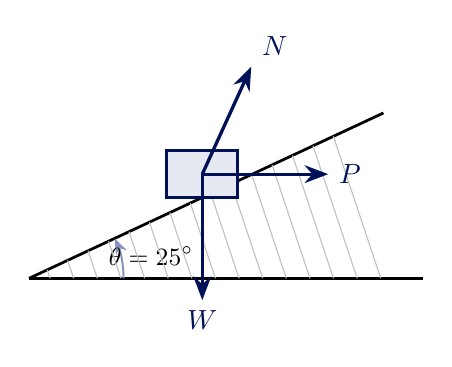
\begin{tikzpicture}
\draw[line width=1pt] (0,0) -- (5,0);
\draw[line width=1pt] (0,0) -- (4.5,2.1);
\draw[dim] (1.2,0) arc (0:25:1.2);
\node at (1.55,0.28) {\small $\theta=25^\circ$};
\begin{scope}
  \clip (0,0) -- (4.5,2.1) -- (5,0) -- cycle;
  \foreach \x in {0,0.3,...,5} {\draw[gray!50, line width=0.4pt] (\x,-1) -- (\x-1,2);}
\end{scope}
\coordinate (P) at (2.3,1.073);
\fill[lightaccent, draw=mainblue, line width=1pt] ($(P)+(-0.55,-0.05)$) rectangle ++(0.9,0.6);
\coordinate (Ctr) at ($(P)+(-0.1,0.25)$);
\draw[force] (Ctr) -- ++(0,-1.6) node[below] {$W$};
\draw[force] (Ctr) -- ++(65.5:1.5) node[above right] {$N$};
\draw[force] (Ctr) -- ++(1.6,0) node[right] {$P$};
\end{tikzpicture}

% ---------- Figure 4: boom and cable supporting a load ----------
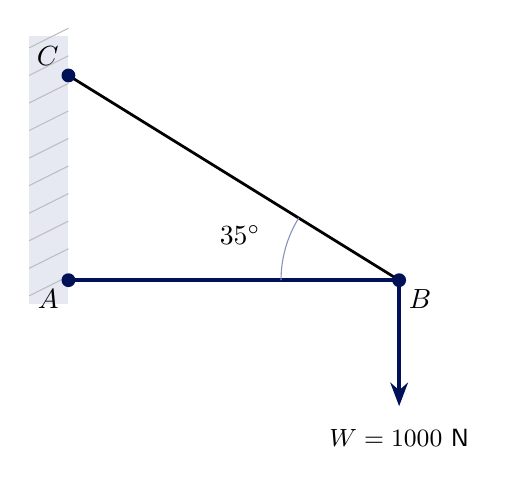
\begin{tikzpicture}
\coordinate (A) at (0,0);
\coordinate (B) at (4.2,0);
\coordinate (C) at (0,2.6);
\fill[lightaccent] (-0.5,-0.3) rectangle (0,3.1);
\foreach \y in {-0.2,0.15,...,3.0} {\draw[gray!50,line width=0.4pt] (-0.5,\y) -- (0,\y+0.25);}
\draw[line width=1.5pt, mainblue] (A) -- (B);
\draw[line width=1pt] (C) -- (B);
\fill[mainblue] (A) circle (2.5pt);
\fill[mainblue] (B) circle (2.5pt);
\fill[mainblue] (C) circle (2.5pt);
\node[below left] at (A) {$A$};
\node[below right] at (B) {$B$};
\node[above left] at (C) {$C$};
\pic[draw=accent, angle radius=15mm, "$35^\circ$", angle eccentricity=1.4] {angle=C--B--A};
\draw[force] (B) -- ++(0,-1.6);
\node at (4.2,-2.0) {\small $W = 1000\ \text{N}$};
\end{tikzpicture}

\end{document}
